\chapter{Implementación}

% La implementación del software se ha dividido en hitos. Estos, han sido definidos en Github
% y cada uno de ellos contiene un grupo de \textit{issues} que se corresponden con las distintas
% mejoras que se han ido incorporando al software a lo largo de su desarrollo.\\

Al inicio del proyecto tenía:
\begin{itemize}
    \item Una placa Redwire Econotag r3.
    \item Un BSP para la Econotag.
    \item Un repositorio de github para el Kernel de FreeRTOS.
    \item Un repositorio de github para el resto de FreeRTOS.
\end{itemize}

\section{Paso 1: Familiarizarse con la estructura de FreeRTOS}
FreeRTOS está dividido en varios repositorios de Github que forman submódulos, pero para este proyecto solo hay dos relevantes: el repositoro principal \href{https://github.com/FreeRTOS/FreeRTOS}{FreeRTOS/FreeRTOS} y el kernel que contiene los ports \href{https://github.com/FreeRTOS/FreeRTOS-Kernel}{FreeRTOS/FreeRTOS-Kernel}.

Para empezar creé un fork en github de los dos repositorios que necesitaba de FreeRTOS. Cloné el repositiorio principal, modifiqué el archivo \textit{.gitmodules} y utilicé el comando \textit{git submodules sync} para que el submodulo \textit{Source/} apuntase a mi fork del kernel. Finalmente inicialicé el submódulo del kernel.

En resumen, esta fué la serie de comandos para clonar y inicializar los repositorios:
\begin{lstlisting}[language=bash]
$ git clone git@github.com:epaubert/FreeRTOS-TFG.git
$ cd FreeRTOS-TFG/
$ sed -i 's/FreeRTOS\/FreeRTOS-Kernel/epaubert\/FreeRTOS-Kernel-TFG/'\
.gitmodules
$ git submodule sync
$ git submodule init FreeRTOS/Source/
$ git submodule update FreeRTOS/Source/
\end{lstlisting}

En siguiente lugar creé los directorios \path{FreeRTOS-TFG/FreeRTOS/Source/portable/GCC/ARM7_MC13224V} y \path{FreeRTOS-TFG/FreeRTOS/Demo/ARM7_MC13224V_GCC} que contendrán el código necesario para el port y la demo respectivamente. Posteriormente copié los archivos plantilla de
La figura \ref{fig:DirsFreeRTOS} muestra un diagrama de los directorios y los archivos.

\begin{figure}%[h]
\centering
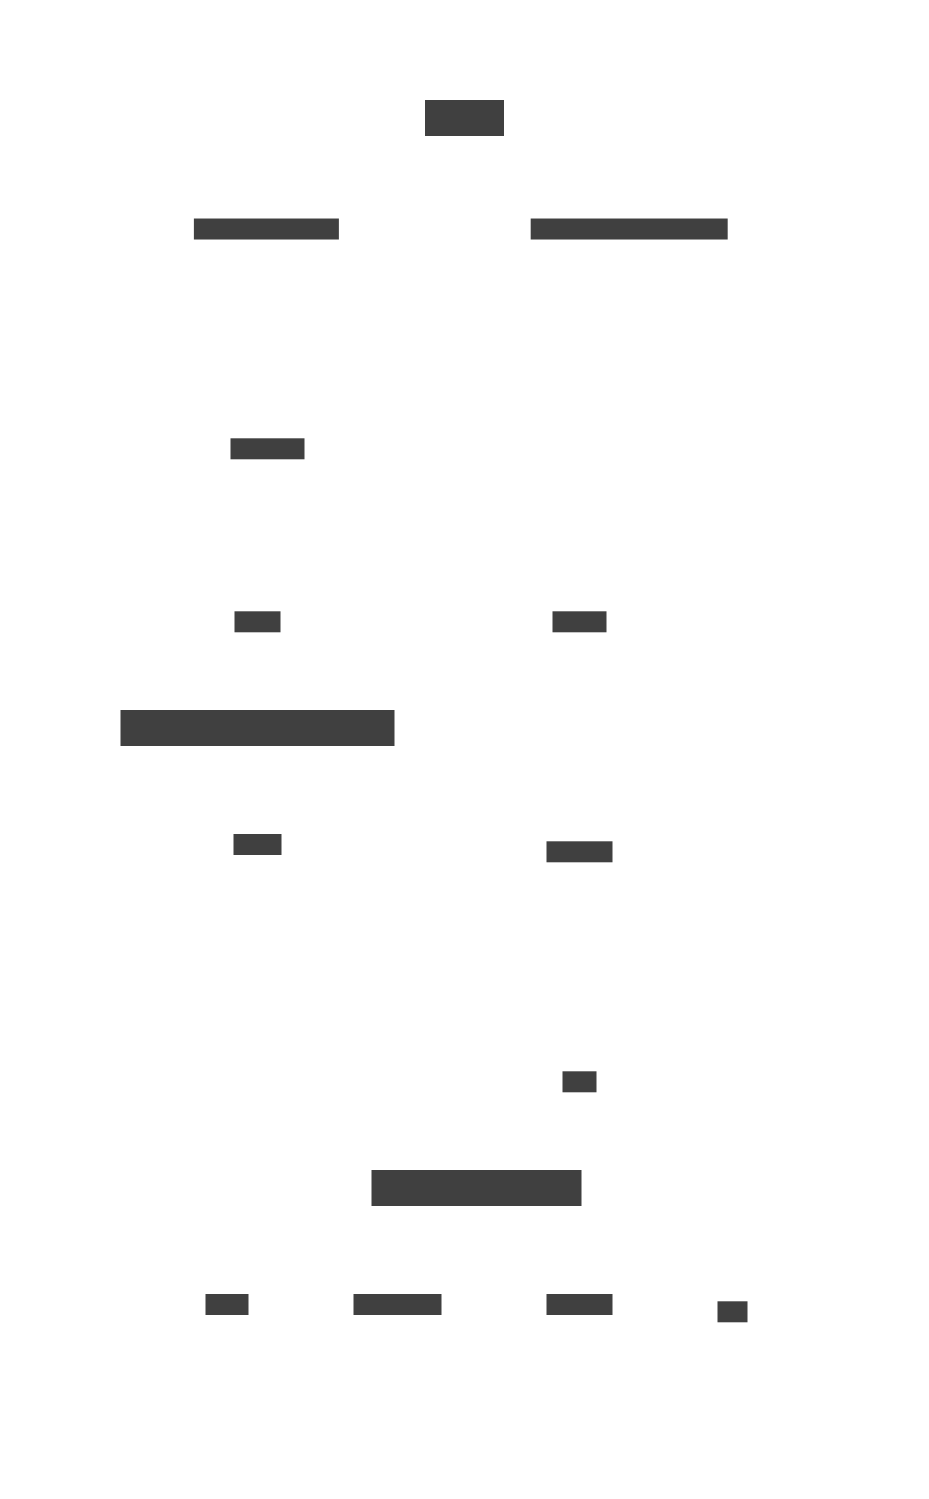
\includegraphics[width=\textwidth]{img/carpetasFreeRTOS.png}
\label{fig:DirsFreeRTOS}
\caption{Estructura de los directorios y archivos de FreeRTOS}
\end{figure}

\section{Paso 2: integración del BSP}
Antes de empezar a implementar dentro de FreeRTOS, decidí integrar el BSP dentro del port para que utilizar las herramientas que ya estaban implementadas en el BSP tango en el port como en la demo.
FreeRTOS utiliza una serie de \textit{Makefiles} para su compilación así que decidí sustituir el \textit{Makefile} del BSP por un \textit{CMakeLists.txt} y así poder incluir la compilación del BSP más orgánicamente en el port.

\section{Paso 3: Ampliación del BSP}
FreeRTOS requiere de interrupciones periódicas para medir el tiempo transcurrido.

\section{Paso 4: }

